\documentclass{standalone}
\usepackage{tikz,color}
\begin{document}

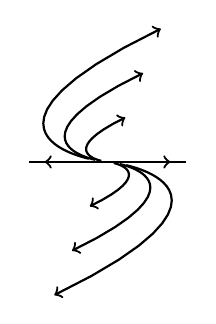
\begin{tikzpicture}
\draw [->, thick] (0,0) to (-0.8,0);
\draw [->, thick] (0,0)  to (0.8,0);
\draw [-, thick ] (-1,0) to (1,0);
\draw [->, thick, domain= -6:0.2, samples=25]
	 plot({0.1*exp(0.6*\x)+0.5*\x*exp(0.6*\x)},{0.5*exp(0.6*\x)});
\draw [->, thick, domain= -6:0.2, samples=25]
	 plot({0.2*exp(0.6*\x)+\x*exp(0.6*\x)},{exp(0.6*\x)});
\draw [->, thick, domain= -6:0.2, samples=25] 
	plot({0.3*exp(0.6*\x)+1.5*\x*exp(0.6*\x)},{1.5*exp(0.6*\x)});
\draw [->, thick, domain= -6:0.2, samples=25] 
	plot({-0.1*exp(0.6*\x)-0.5*\x*exp(0.6*\x)},{-0.5*exp(0.6*\x)});
\draw [->, thick, domain= -6:0.2, samples=25]
	 plot({-0.2*exp(0.6*\x)-\x*exp(0.6*\x)},{-exp(0.6*\x)});
\draw [->, thick, domain= -6:0.2, samples=25] 
	plot({-0.3*exp(0.6*\x)-1.5*\x*exp(0.6*\x)},{-1.5*exp(0.6*\x)});

\end{tikzpicture}
\end{document}
